\newpage
\section{Abstract}

\subsection*{Introduction}

It’s becoming clear that the livestock farming sector is one of the main contributors to the world’s water depletion, land use, biodiversity loss and greenhouse gas emissions. Over a third of the world’s crop calories are used as animal feed, and only a third of those feed calories end up contributing to the human diet. [https://iopscience.iop.org/article/10.1088/1748-9326/8/3/034015] With trends in global consumption and production of meat growing, the impacts of livestock farming are set to grow.
Alternative protein developments aim to substantially reduce the impact of feeding the human and domesticated animal population of the world by substituting the billions of animals grown and slaughtered every year with an alternative. There are significant developments in the plant-based, microbial, and fermented protein research, but we focus on evaluating the viability of directly substituting reared and slaughtered cattle with commercially cultured beef. 

% \begin{figure}[h]
%     \centering
%     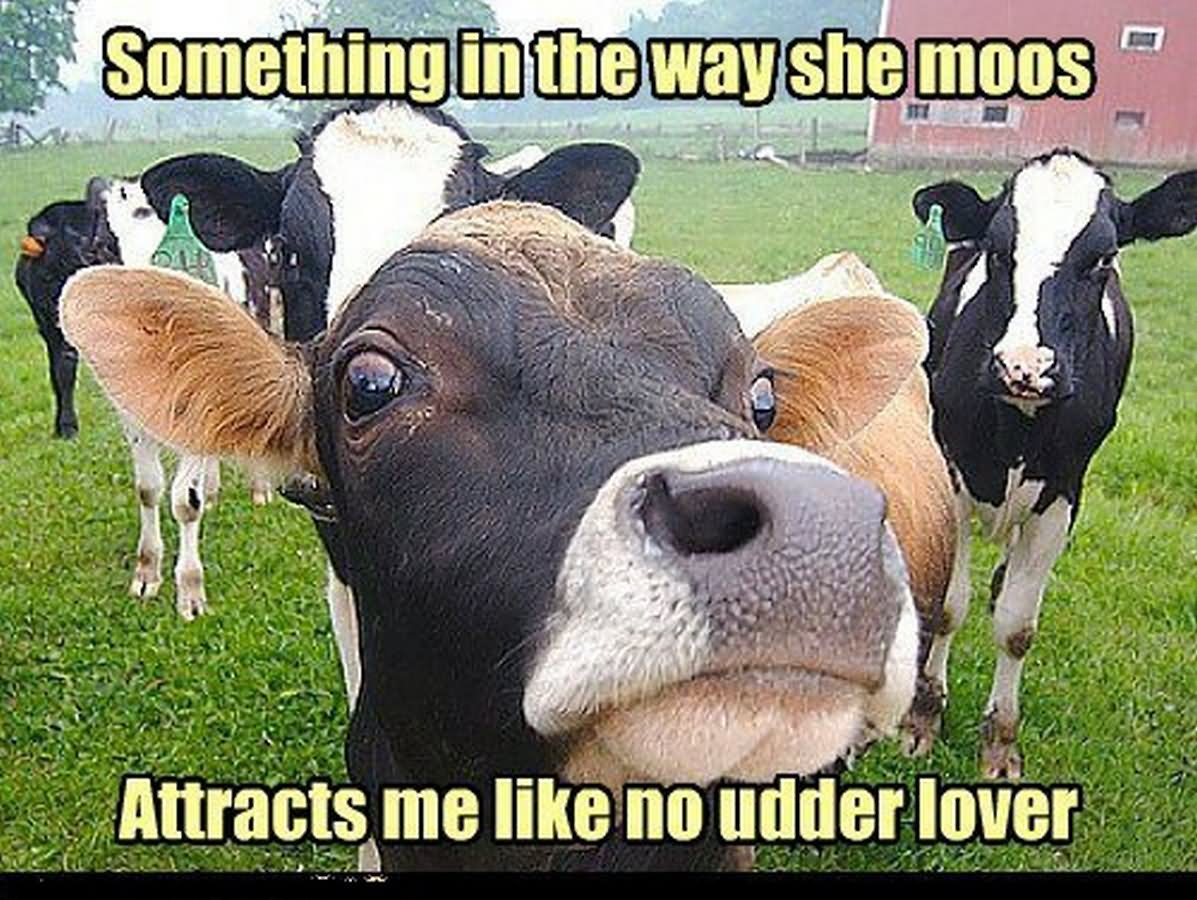
\includegraphics[width=0.75\textwidth]{will/example-image.jpg}
%     \hfill
%     \caption{An example image \citet{E-Cannon2022}}
%     \label{fig:example-image}
% \end{figure}

\subsection*{Summary}

Whilst shifting crop use away from animal feed could feed an additional 4 billion people and reduce global Green House Gas emissions by about a tenth, our venture proposal wouldn’t be profitable in today’s political and economic climate. [https://iopscience.iop.org/article/10.1088/1748-9326/8/3/034015] [https://www.sciencedirect.com/science/article/pii/S0377840111001933 MAKE SURE TO ACCOUNT FOR INCREASE IN CROP CONSUMPTION]
Unless commissioned by a special interested party – the outgoings and capital cost, along with risk associated with such a new, volatile and saturated market – mean that the proposal is unlikely to work better than other protein alternatives. If policies were introduced that reduced the subsidies on traditionally farmed meat and moved them to cultured meat, then our proposal might gain more traction to feed demand as our prices ease. [https://www.oxfordmartin.ox.ac.uk/blog/meat-and-dairy-gobble-up-farming-subsidies/]

% Example equation \ref{eq:example-equation}.

% \begin{equation}
%     beef_{moo} = fear^{10}
%     \label{eq:example-equation}
% \end{equation}

% Example list:

% \begin{itemize}
%     \item \(\bm{X} \in \mathbb{R}^{n \times p}\), a matrix containing the scrutinised data-points $\bm{x} \in \mathbb{R}^{p}$ from each sample,
%     \item \textit{regression\textunderscore targets}, known as $\bm{\bar{y}}\in \mathbb{R}^n$, is a vector containing the regression targets for the samples (individually known as $\Bar{y}$), and
%     \item \textit{class\textunderscore labels} $\in \{1,\dots,p\}$ which keeps track of which Gaussian each sample came from (a target for classification).
% \end{itemize}

% Example table \ref{table:1}

% \begin{table}[!ht] % the [h] forces the table to be "here". This is quite a short document so LaTeX struggles to find a nice arrangement for the floats! Not normally needed
%     \begin{center}
    
%         \begin{tabular}{|l|c|c|} 
%             \hline
%             \textbf{learning\_rate} & \textbf{mse\_train} & \textbf{mse\_val} \\ 
%             \hline
%             1e-05&1.1254&1.1747\\
%             \hline
%             0.0001&0.31296&0.3012\\
%             \hline
%             0.001&0.095492&0.088045\\
%             \hline
%             0.01&0.046835&0.052905 \\
%             \hline
%             0.1&0.046534&0.052771\\
%             \hline
%             1&NaN&NaN \\
%             \hline
%         \end{tabular}
%         \caption{Table of Mean Squared Difference from different learning rates.}
%         \label{table:1}
            
%     \end{center}
% \end{table}

% Example aligned equation:

% \begin{align*}
%     \mathcal{L}_c &= -ylog(\bar{y}) - (1-y)log(1-\bar{y})\\
%     &= ylog(1+e^{-\bm{\hat{x}^T\theta}})-(1-y)log(\frac{e^{-\bm{\hat{x}^T\theta}}}{1+e^{-\bm{\hat{x}^T\theta}}})\\
%     &=(y-y)log(1+e^{-\bm{\hat{x}^T\theta}})-(1-y)log(e^{-\bm{\hat{x}^T\theta}})+log(1+e^{-\bm{\hat{x}^T\theta}})\\
%     &=(1-y)\bm{\hat{x}^T\theta}+log(1+e^{-\bm{\hat{x}^T\theta}})\\
%     \Delta_{\bm{\theta}}\mathcal{L}_c &=(1-y)\bm{\hat{x}}-\frac{e^{-\bm{\hat{x}^T\theta}}}{1+e^{-\bm{\hat{x}^T\theta}}}\bm{\hat{x}}\\
%     &=(1-y)\bm{\hat{x}}-(1-\bar{y})\bm{\hat{x}}\\
%     &=\bm{\hat{x}}(\bar{y}-y)
% \end{align*}

% END OF TEMPLATE